\chapter{Learning LaTeX and R}


\section{Learning LaTeX}
This section belatedly covers one of the key challenges and skills gleaned through and during the PhD. Learning adequate latex skills is a key factor in being able to publish research, yet seldom covered at my university, nor at many other institutions according to others informally.
As someone who has been working with developing and testing software, aspects of the experience were already familiar, for instance the use of markup commands, the separation of content and appearance, and so on. And yet, learning even the basics took a while. 

The source code of this thesis is littered with comments containing notes and links to various sources of clues on using latex, and I am no master of the topic.

Getting started? here's one place to do so~\url{https://olivierpieters.be/blog/2015/09/21/introduction-to-latex}

As one of the TeX FAQ articles states~\emph{``Tables and figures have a tendency to surprise, by floating away from where they were specified to appear."}~\citep{texfaq_floats}.

The following answer is simply pivotal in my understanding of how figures and tables, etc. (all considered `floats' in LaTeX) are placed in a typeset document~\href{https://tex.stackexchange.com/questions/39017/how-to-influence-the-position-of-float-environments-like-figure-and-table-in-lat/39020#39020}{LaTeX floats terminology}. I now need to consider how I can use this information to improve the positioning of my tables and figures in this thesis. 

Positioning of floats close to their location in the text is also clearly and succinctly covered in the answer on tex stackechange~\href{https://tex.stackexchange.com/a/2282/88466}{Easing the float placement by options}.

The LaTeX project team have written, assembled, and published a wide range of materials on the topic which may well help~\citep{publications_by_the_LaTeX_project_team}. As an example, the previous answer on the tex stackechange site is written up as a document~\href{https://www.latex-project.org/publications/2014-FMi-TUB-tb111mitt-float-placement.pdf}{How to influence the position of float environments like figure and table in LaTeX?}

See also:
\begin{itemize}
    \item \href{https://tex.stackexchange.com/questions/2651/should-i-use-center-or-centering-for-figures-and-tables}{Should I use center or centering for figures and tables?}
    \item \url{https://olivierpieters.be/blog/2015/11/11/tables-in-latex} and~\url{https://olivierpieters.be/blog/2015/10/23/latex-plotting-from-file} also might help if I decide to load data from CSV files into plots or tables.
    \item \url{https://en.wikibooks.org/wiki/TeX/def} and~\url{https://en.wikibooks.org/wiki/TeX/let}
\end{itemize}

Learning about the preamble (the latex configuration file and similar info in the thesis.tex file) is usefully described in~\url{https://olivierpieters.be/blog/2016/08/10/latex-preamble}. 

Making sense of various commands, and in particular~\texttt{\\let} was another challenge that I struggled to find explanations for,~\citep{tex_stackechange_let_and_def} unlocked this topic for me -~\texttt{\\let} provides a synonym for an existing command,~\texttt{\\def} defines a new command. See also~\url{https://olivierpieters.be/blog/2016/09/09/defining-new-latex-macros} for additional context and examples of~\texttt{\\newcommand} which is recommended in place of~\texttt{\\let}.

\subsection{Citations, references, and so on}

\begin{itemize}
    \item \href{https://tex.stackexchange.com/questions/14155/recreating-biblatex-option-autocite-footnote-style-verbose-trad1-in-bibtex}{recreating biblatex option autocite=footnote,style=verbose-trad1 in bibtex} I hope I never need this. It's for if/when I try to adapt and adopt Ralf Jung's thesis template, and just might help me when I'm trying to improve the format of my bibliography.
    \item Ditto,~\href{https://tex.stackexchange.com/questions/58576/autocite-footnote}{autocite=footnote} is something Ralf uses with biblatex.
    \item \href{https://tex.stackexchange.com/questions/5091/what-to-do-to-switch-to-biblatex}{What to do to switch to biblatex?} has an illuminating answer:~\url{https://tex.stackexchange.com/a/5105/88466}.
    \item Some great practical tips on using citations in the text are documented online by John Owens here~\url{https://www.ece.ucdavis.edu/~jowens/biberrors.html} and in~\url{https://freedom-to-tinker.com/2011/02/25/public-service-rant-please-fix-your-bibliography/}.
    \item an \texttt{@url\{\}} bibliography entry? see~\url{https://nxg.me.uk/dist/urlbst/} for details, however this is from 2011 and might be out of date now.
    \item A rant on fixing the bibliography~\url{https://freedom-to-tinker.com/2011/02/25/public-service-rant-please-fix-your-bibliography/}
    \item A couple of articles on using BibTeX, the first~\url{https://libguides.rhul.ac.uk/referencing/latex} cites the second, more comprehensive guide~\url{https://www.latex-tutorial.com/tutorials/bibtex/}.
    \item Overleaf's overview on \texttt{natbib} which I'm currently using~\url{https://www.overleaf.com/learn/latex/bibliography_management_with_natbib}.
\end{itemize}

\subsection{Formatting}
Formatting long URLs is not well done in the current template. I've added a \texttt{\\urlstyle{sf}}, based on the following article (\url{https://www.joachim-breitner.de/blog/519-Nicer_URL_formatting_in_LaTeX}). It may be worth trying out their more sophisticated approach once I've revised my template to the Tufte style one. 

\section{Learning R}

The R language, and the popular IDE R Studio, have provided a productive environment for data analysis and graphing. In terms of my research, they are part of my objective to share the code and analysis in conjunction with the thesis and the underlying data.

Automated Data Collection with R~\cite{munzert2014automated} is an interesting, relevant book with several useful examples\footnote{\url{http://www.r-datacollection.com/}}. However the world has moved on since the book was written and published so some of the examples need updating and enhancing.

Other resources include the RStudio cheatsheets~\footnote{\url{https://rstudio.com/resources/cheatsheets/}} and online courses on the datacamp.com website~\footnote{\url{https://learn.datacamp.com/}}.

\section{Using R for reproducible research}
An aptly titled book, \emph{Reproducible research with R and R studio}, now in its third edition~\cite{gandrud2020reproducible} provides a useful model for my research and analysis. Accordingly, the source code for my analysis using R is available in an opensource project on GitHub \url{https://github.com/julianharty/gpc-report-analysis}. Publishing the code facilitates reproducibility and enables others to use, critique, and improve the code.

\begin{lstlisting}[caption=Parsing dates from Wikipedia content,label=listing:parse_dates]
> yend_clean <- str_extract_all(danger_table$yend, "^[[:digit:]]{4}")
> danger_table\$yend <- as.numeric(yend_clean)
> danger_table$yend

  [1] 2001 1992 2013 2013 2013 2013 2016 2016 2016 2003 1986 2014
 [13] 2005 2013 2003 2013 1993 2012 1984 2015 2017 2016 2017 2000 
 [25] 2019 1997 2018 2012 1997 2002 2006 1992 2016 2007 1997 1982
 [37] 2015 2016 2016 2014 2015 2010 1996 2016 1999 2007 2014 2013
 [49] 2012 2012 2010 2011 1994
\end{lstlisting}

\section{Quality Control Tools: Implemented in R}
There are various visually-oriented quality tools, including Ishikawa diagrams. The \texttt{SixSigma} package can be used to create these diagrams using R code, as discussed in an interesting article \emph{7 Basic Quality Tools with R}~\cite{7_basic_quality_tools_with_R}.

Another relevant reference is \emph{Quality Control in R}~\cite{quality_control_in_R_book}. Chapter 3 \emph{The Seven Quality Control Tools in a Nutshell: R and ISO Approaches} discusses these same tools in greater depth and rigour. The authors also provide a website with an R package~\url{http://www.qualitycontrolwithr.com/package.html} and their example appears to predate and inspire the one references in~\cite{7_basic_quality_tools_with_R}.

\subsection{Ishikawa Diagrams}
As discussed in the Related Work chapter, Ishikawa diagrams can hep identify causes and effects visually so they can be considered and the issue addressed.

\begin{lstlisting}
# Import the SixSigma package
library(SixSigma)

# Specify the effect to be analyzed
b.effect <- "Delay"

# Create a vector with the names of the causes classification groups
b.groups <- c("Personnel", "Weather", "Suppliers", "Planning")

# Create a vector that contains the causes
b.causes <- c(vector(mode = "list", length = length(b.groups)))

# Create lists corresponding to the causes for each corresponding group
b.causes[1] <- list(c("Training", "Inadequate"))
b.causes[2] <- list(c("Rain", "Temperature", "Wind"))
b.causes[3] <- list(c("Materials", "Delays", "Rework"))
b.causes[4] <- list(c("Customer", "Permissions", "Errors"))

# Create the cause-and-effect diagram
ss.ceDiag(b.effect,
          b.groups,
          b.causes,
          main = "Cause-and-Effect Diagram (SixSigma package)",
          sub = "Construction Example")
\end{lstlisting}
Source code reproduced from GitHub, and \href{https://gist.github.com/rsalaza4/eff4a0a7e8e4894e4b82152fcf66e847/raw/cfbfe93c784989ee8fd6b686dd26fb88f4cec26d/Cause-and-effect\%20diagram.R}{available online}. This generates the functional diagram shown in Figure ~\ref{fig:ishikawa-example-in-R}.

\begin{figure}[htbp!]
    \centering
    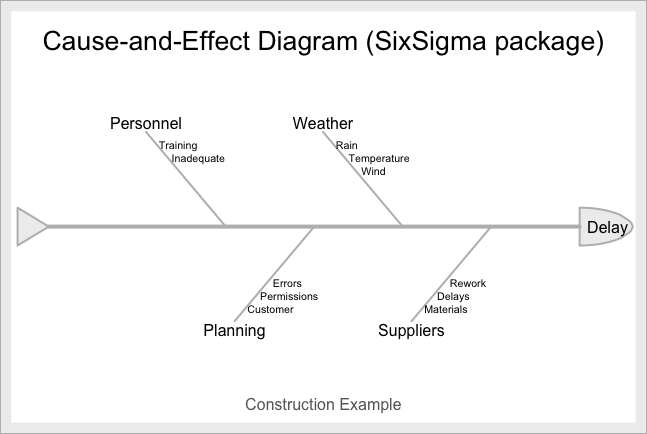
\includegraphics[width=0.8\textwidth]{images/cause-effect-diagram.png}
    \caption{Cause and Effect diagram generated by R code}
    \label{fig:ishikawa-example-in-R}
\end{figure}

\hypertarget{pareto.diagrams.in.r}{}
\subsection{Pareto Diagrams}
Some issues have greater effects than others, and potentially those with the greatest effects are worth addressing first in order to maximise the measured improvement \emph{e.g.} in software quality.

The \texttt{qcc} R library enables Pareto figures, such as Figure~\ref{fig:pareto_chart_example}, to be generated in R~\cite{7_basic_quality_tools_with_R}. 

\begin{lstlisting}
# Import the qcc package
library(qcc)                  

# Create a vector with the number of defects per defect type
defects <- c(27, 389, 65, 9, 15, 30, 12, 109, 45, 321)            

# Create a vector with the names of the defects 
names(defects) <- c("Defect 1", "Defect 2", "Defect 3", "Defect 4",
                    "Defect 5", "Defect 6", "Defect 7", "Defect 8",
                    "Defect 9", "Defect 10")   

# Create the Pareto chart
pareto.chart(defects,
             ylab = "Frequency",
             y2lab ="Cumulative Percentage",
             main = "Pareto Chart",
             cumperc = seq(0, 100, by = 20))
\end{lstlisting}
\href{https://gist.githubusercontent.com/rsalaza4/a69615daba7c7c56290838b46cc121cc/raw/974774009f38d6af534168f2a324ce2b3c61d632/Pareto\%20chart.R}{Code Gist for Pareto chart.R}
\begin{figure}[htbp!]
    \centering
    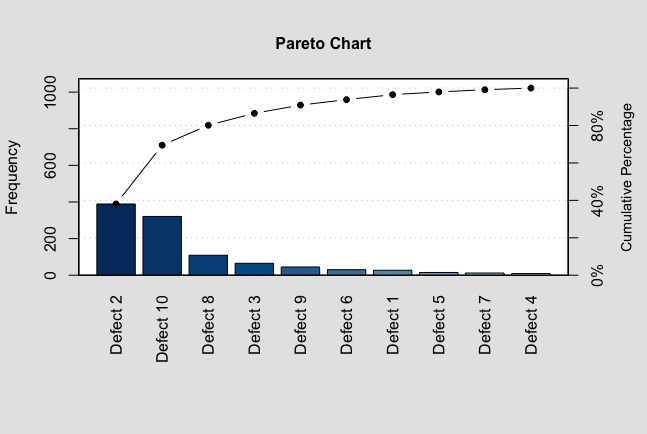
\includegraphics[width=0.8\textwidth]{images/Pareto_chart_example.png}
    \caption{Pareto Chart example}
    \label{fig:pareto_chart_example}
\end{figure}

